\chapter{Origami-inspired Mesostructures}
\label{ch:origami_ribbon}
\graphicspath{{origami_ribbon/fig/}}

This chapter is based upon the joint work: Y. Li, S. J. Avis, T. Zhang, H. Kusumaatmaja, and X. Wang, ``Tailoring the multistability of origami-inspired, buckled magnetic structures via compression and creasing'', \emph{Mater. Horiz.}, 8, 3324 (2021).

In particular, the experimental ferromagnetic structures are the work of Y. Li, while the simulations and energy landscape analysis are my own work.



\section{Introduction}

Origami, the ancient art of folding two-dimensional (2D) thin sheets along predefined creases to create three-dimensional (3D) objects\cite{Chen2015,Dudte2016,Ning2018}, has inspired the design of many engineering structures for a wide range of applications, including deployable systems\cite{Thesiya2015,Melancon2021,Liu2020}, self-folding machines\cite{Felton2014}, reconfigurable metamaterials\cite{Silverberg2014,Chen2021,Yang2019}, and DNA origami\cite{Hellmeier2021}.
For those applications, a key design feature of the structures is their ability to have multiple stable states as well as the tailoring of those states for tunability and adaptability.
Existing works so far have primarily focused on bistable systems for rigid origami patterns (like the Miura folding\cite{Miura1985} and its derivatives\cite{Filipov2015}) and deformable origami (like the twisted square pattern\cite{Silverberg2015}).
For example, Sadeghi and Li realised rapid and reversible folding by harnessing the asymmetric bistability of designed origami structures\cite{Sadeghi2020}.
Liu et al. demonstrated that a folded hypar origami, obtained by folding a piece of paper along concentric squares and their diagonals to arrive at a seemingly smooth saddle shape, exhibits bistability between two symmetric configurations\cite{Liu2019b}.
More recently, Melancon et al. realised pressure-deployable origami structures characterised by two stable configurations — one compact and one expanded – at the meter scale\cite{Melancon2021}.
Furthermore, Fang et al. showed that the potential energy landscapes of stacked Miura-ori and the Kresling-ori structures, and therefore their stability profiles and constitutive force–displacement relations, can be effectively tuned by embedded magnets\cite{Fang2019}.

In addition to multistability, reconfiguration among the different stable states of origami-inspired structures in a well-controlled manner is demanded in many engineering devices and structures.
Theoretical and experimental studies have been performed on reconfiguration paths in origami-inspired structures.
For example,  Zhai et al. created an origami-inspired mechanical metamaterial that can be deployed and collapsed along different configuration paths\cite{Zhai2018}.
Silverberg et al. showed that hidden degrees of freedom in square twist origami structures give rise to a critical transition from mono- to bi-stability\cite{Silverberg2015}.
Moreover, significant advances have been made to improve the tunability and adaptability of origami-inspired structures by incorporating stimuli-responsive materials, which provides opportunities for micro robotics, biomedical devices, and many others\cite{Jamal2013,Chen2020,Xu2017,Novelino2020,Xu2017a}.

Previous studies have laid solid foundations for the design and development of origami-inspired structures with bistability and tunability.
One of the remaining challenges in this field is to actively control the number of possible stable states and their reconfiguration paths.
Here we investigate this by extending our studies of mesostructures from the previous chapter to incorporate origami-inspired creases, which can increase the prevalence of multistable states.
There are innumerable structures that can be constructed from networks of creased ribbons, so we instead restrict our attention to the most simple structure, a single ribbon with multiple creases, to gain fundamental insights about the effect of creases on multistability.
However, the same approaches could also be applied to study other structures.

The two key parameters that we control are compressive strain and creasing in the ribbon, which are selected because they are easy to tune and very effective to alter the multistable behaviors of the structure for real applications.
We utilise a similar computational approach as the last chapter in order to construct phase diagrams showing how the available states sensitively depend on the compressive strain and the number of creases.
Then we generate the the reconfiguration pathways to understand the stability of the various states and how they can interchange upon applying an external magnetic force or varying the applied strain.

Finally, guided by this analysis, our collaborators have produced diverse complex origami-inspired structures, including structure arrays that be individually tuned based on the multistability of the structural unit and a biomimetic insect.



\section{Results and Discussion}

\subsection{Concept of origami-inspired, multistable magnetic structures}

\Cref{fig:or-1} schematically illustrates the experimental assembly process and reconfiguration of origami-inspired structures compressively buckled from ferromagnetic composites\cite{Wang2019a,Zhang2015,Liu2019}.
These are constructed using the approach described in \cref{ch:mesostructures}, however laser patterning is also used in order to create crease sections with a thickness that is 46.15\% of the non-crease regions.
Due to this reduced thickness, the crease regions act as flexible hinges that can bend into different states, affecting the potential multistable reconfigurations\cite{Tang2019}.

Under an external magnetic field generated by a manually manipulative magnet, the assembled origami-inspired structure can be reconfigured into up to four distinct stable states: state 1 (S1, one center peak), state 2 (S2, one side peak), state 3 (S3, two peaks), and state 4 (S4, twisted two peaks).
These are then able to remain stable after the removal of the applied magnetic field.

\begin{figure}
  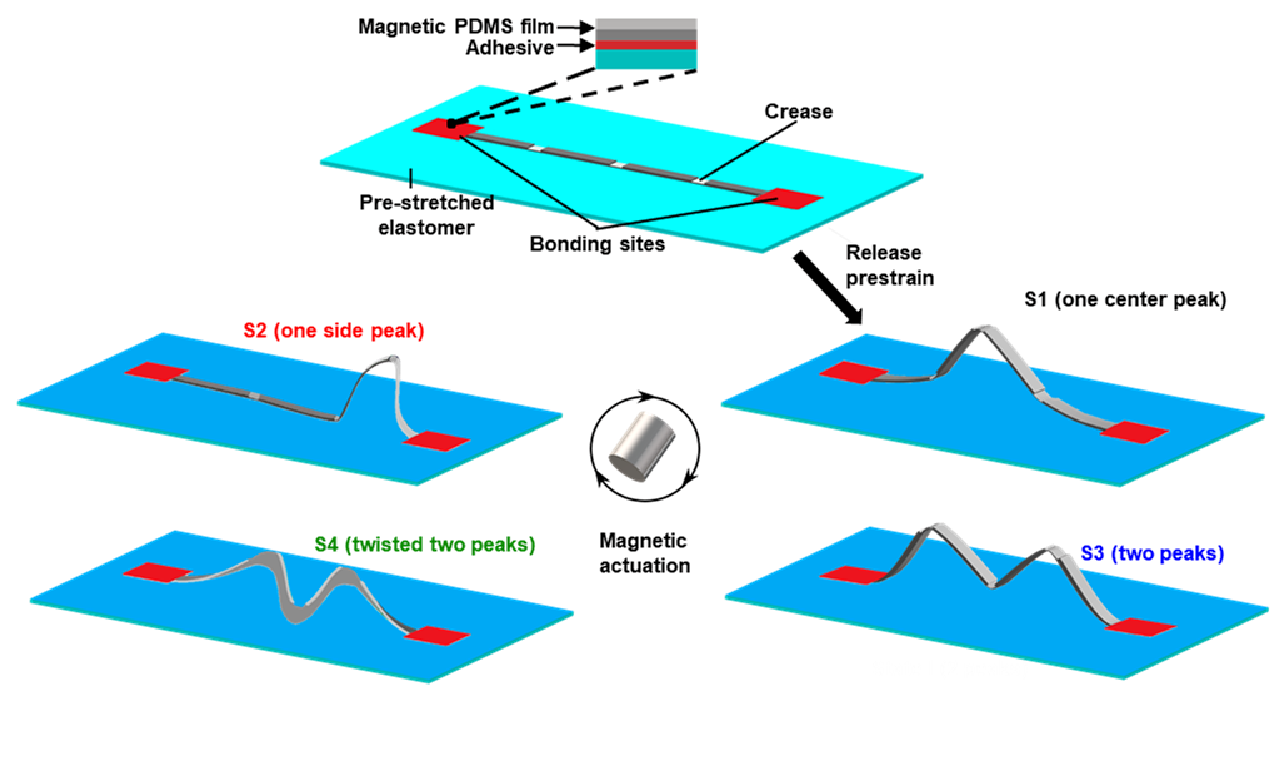
\includegraphics[width=\textwidth]{figure_1.pdf}
  \caption{
    Schematic illustration of the assembly and magnetic reconfiguration schemes of multistable origami-inspired ribbon structures.
  }
  \label{fig:or-1}
\end{figure}


\subsection{Phase diagram of stable states for origami-inspired structures}

We first study the effect of two essential parameters, the number of creases and compressive strains, on the number and configurations of stable states by using a ribbon structure as an example.
A phase diagram, indicating the stable states of the structure with up to seven creases and at strain levels of 0\%-40\%, is shown in \cref{fig:or-2}(a) and serves as a theoretical foundation for the multistability design.
The phase diagram is constructed computationally by identifying the local minima in the energy landscape of the structure under various conditions of strain levels and crease numbers.

As in \cref{ch:mesostructures}, we have used the discrete shell model, this time with two thicknesses: \SI{130}{\micro\meter} and \SI{60}{\micro\meter}, combined with a random search algorithm for energy minimisation.
At selected points (typically 5 different strain levels for each crease number) across the phase diagram, the structure is randomly initialised several hundreds of times and relaxed to the minima.
Once the qualitatively distinct configurations are identified, we systematically vary the compressive strain to observe the full range over which each state is stable.
It is worth noting that while it is difficult to guarantee that all possible stable states have been obtained, we are unable to find additional states when more points in the phase diagram are sampled.
Hence, we consider the identified stable states to be representative in this study.

\begin{figure}
  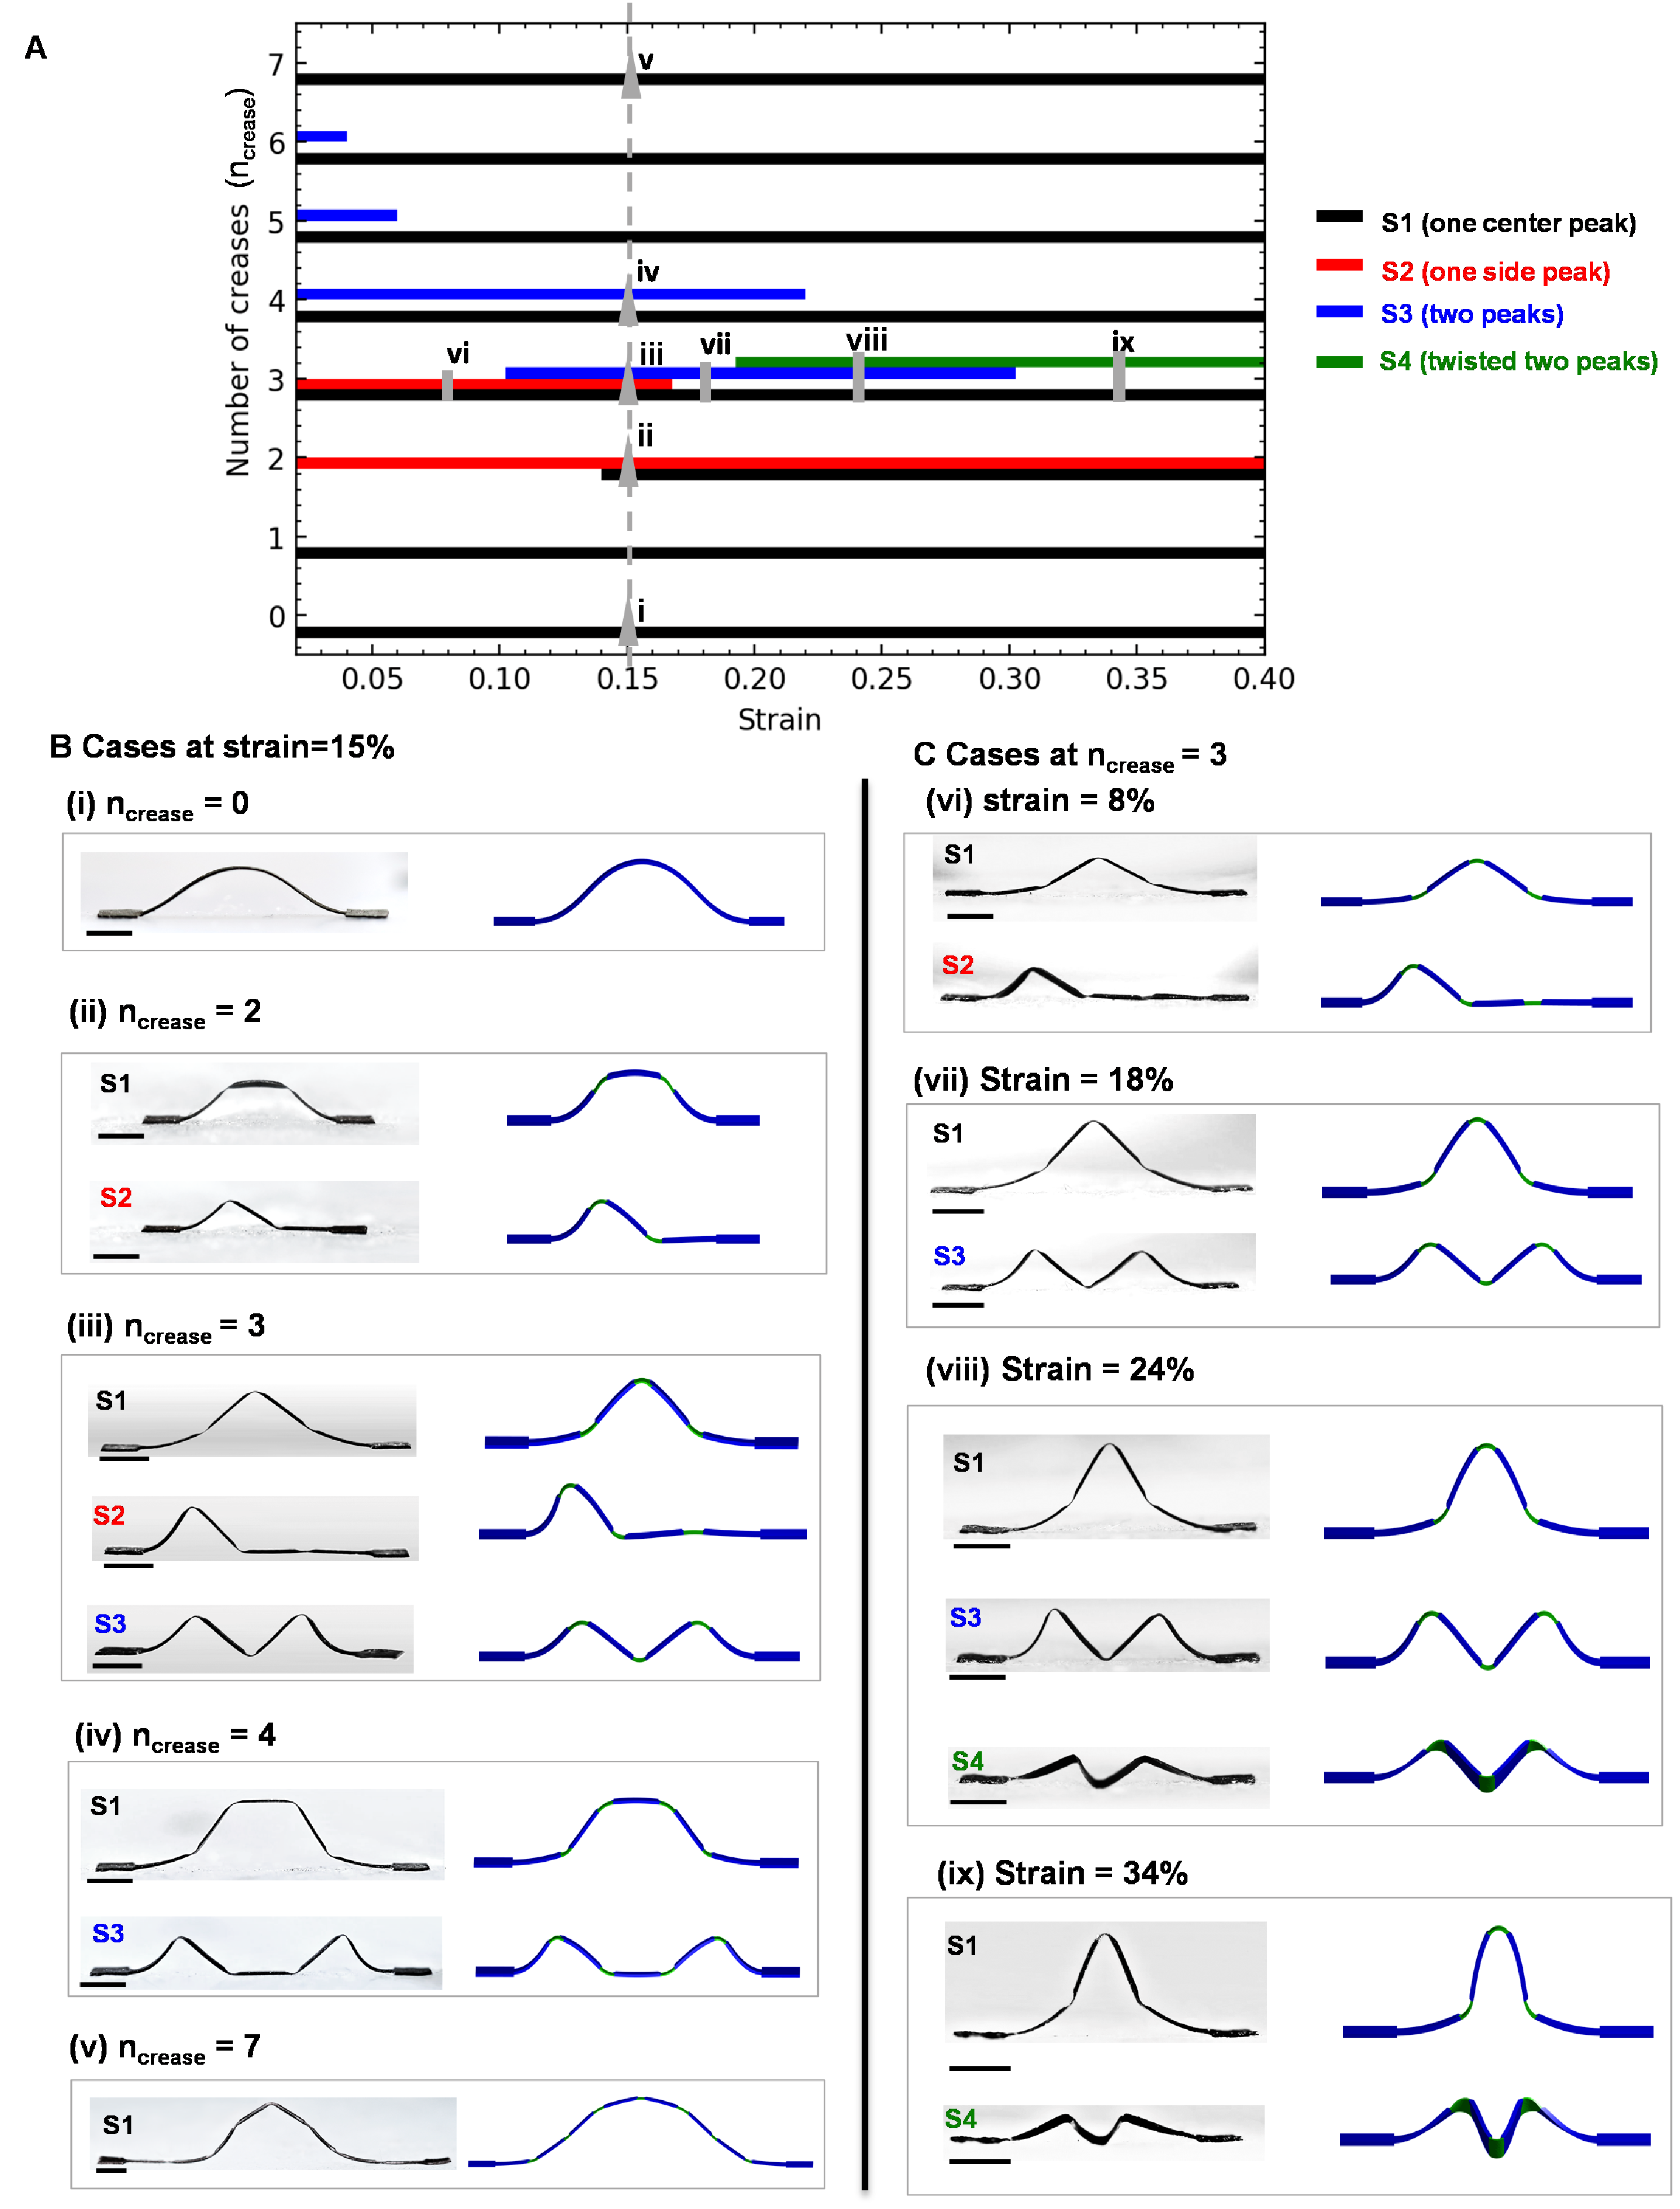
\includegraphics[width=\textwidth]{figure_2.pdf}
  \caption{
    Multistability of origami-inspired ferromagnetic ribbon structures under varying creases and compressive strains.
    (A) Design phase diagram showing the effect of the crease number and compressive strain on the number and configurations of distinct stable states of the ribbon.
    (B) Experimental and computational results of multistable states under a constant strain of 15\% and varying crease numbers, corresponding to points i-v labelled in \cref{fig:or-2}(a).
    Scale bars, 2 mm.
    and (C) Experimental and computational results of multistable states at a constant number of creases ($n_\text{crease} = 3$) and varying strain levels, corresponding to points vi-ix in \cref{fig:or-2}(a).
    Scale bars, 2 mm.
  }
  \label{fig:or-2}
\end{figure}

As shown in \cref{fig:or-2}(a), the number of creases ($n_\text{crease}$) has notable effects on the number and configurations of stable states.
To better illustrate this point, we demonstrate the available states of structures as $n_\text{crease}$ is increased from 0 to 7 under a constant compressive strain of 15\% in \cref{fig:or-2}(b), with the computational and experimental results shown side by side.
When the $n_\text{crease}$ is zero, i.e., the continuous ribbon structure, only S1 (one center peak) exists at all strain levels (e.g., point i).
An additional asymmetric state S2 becomes available when $n_\text{crease}$ rises to two at a compressive strain of 15\% (point ii).
A further increase to three creases causes the structure to admit state S3 (two peaks) at a strain of 15\% (point iii) and S4 (twisted two peaks) at a higher strain level.
As $n_\text{crease}$ increases above three, the number of stable states begins to decline, with S2 becoming unstable for structures with four creases (point iv).
For structures with five creases and above, only S1 remains stable at a compressive strain of 15\%, although S3 is still stable under lower strains for $n_\text{crease}=5$ and 6.
This can be expected because we are approaching the continuous case when the number of creases is large.

The available stable states also depend strongly on the magnitude of the applied compressive strain used in the assembly process of the structure.
We illustrate this using a structure with three creases due to its rich phenomena.

Based on the number and configurations of stable states, five regimes are identified: a) two distinct stable states (S1 and S2; 0-10\% strain), b) three distinct stable states (S1, S2, and S3; 10-17\% strain), c) two distinct stable states (S1 and S3; 17-19\% strain), d) three distinct stable states (S1, S3, and S4; 19-30\% strain), and e) two distinct stable states (S1 and S4; 30-40\% strain).
\Cref{fig:or-2}(c) shows experimental and computational results of distinct stable states at representative strain levels for the five regimes.
Under a relatively low compressive strain of 8\% (point vi), states S1 (one center peak) and S2 (one side peak) exist, which can be reversibly reconfigured into each other via manually controlling the magnetic force and direction.
Increasing the strain to 15\% (point iii) leads to the appearance of a third state, S3 with two peaks, which increases the number of stable states to three.
However, when the strain is further increased to 18\% (point vii), S2 with one side peak disappears.
Further increasing the strain to 24\% (point viii) causes the formation of an interesting twisted state (S4) and therefore increases the number of stable states to three (S1, S3 and S4).
As the strain becomes even larger, S3 disappears and only S1 and S4 exist at the strain of 34\% (point ix).

The experimental and computational results shown above agree reasonably well.
The discrepancy in the configuration of some stable states (e.g., (v) S1 in \cref{fig:or-2}(b)) between experiments and modeling likely results from the adhesion and friction between the structure and the substrate in experiments, which is neglected in computational modeling.
The effect of friction will be further discussed in \cref{sec:or-paths}.

Furthermore, by continuously changing the strain levels from 0\% to 40\% using the 3-crease structure, we record the dynamic progression of the five regimes and the fast, remote magnetic reconfiguration among the stable states within each regime in \cref{vid:ribbon-progress}, which is highly consistent with the predictions of the phase diagram in \cref{fig:or-2}(a).
We also show that the states are stable under perturbations perpendicular to the vertical surface (along the height direction) of the ribbon, except in cases where S4 (twisted two peaks) is present.

The studies above provide important guidelines for tailoring the number and configurations of stable states in origami-inspired structures by tuning the number of creases and the assembly strain.
For example, for applications like digital logics where multiple stable states are desired, structures with three creases may offer more design space and tunability, while structures with a lower or higher number of creases is preferred for applications where a single stable state is needed.

Furthermore, from the phase diagram, we observe that structures with two and three creases have multistable states under a wide range of strain (15\%-40\% strain for the case of two creases and 0\%-40\% strain for the case of three creases), which can be used for applications of multistable structures that demand a wide working strain range.

\subsubsection{Effect of crease thickness and length}
As a brief aside, we also study the effects of modifying the crease thickness ratio and length ratio (defined with respect to the length of each flat segment) on the multistability.
For this, the 3-crease ribbon under a strain level of 14\% is used as an example.

\begin{table}[htb]
  \setkeys{Gin}{width=\linewidth}
  \begin{tabularx}{\textwidth}{CCCCC}
    \hline\hline
    Thickness ratio & State 1 & State 2 & State 3 & State 4 \\
    \hline
    0.67 & 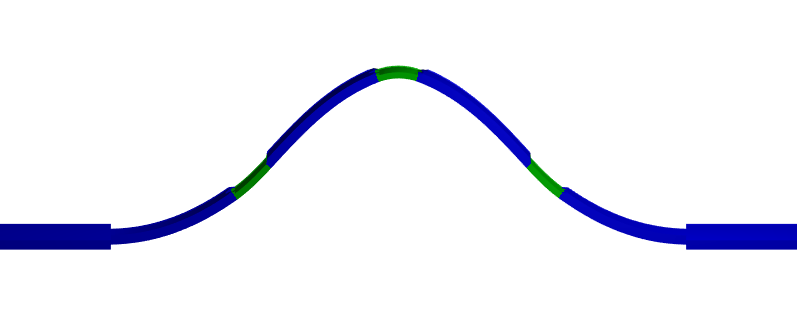
\includegraphics{tratio/1-0.67.png} & \xmark                              & \xmark                          & \xmark \\
    0.56 & 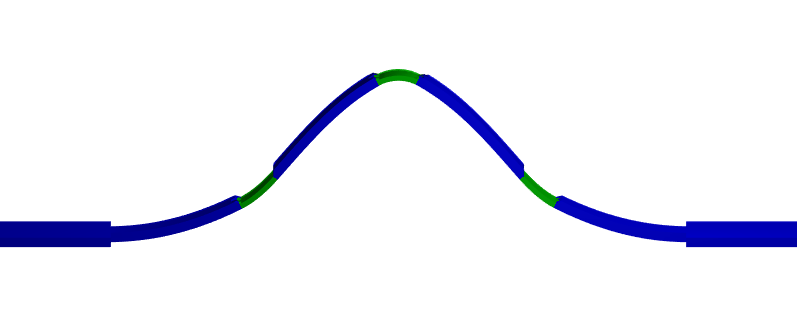
\includegraphics{tratio/1-0.56.png} & 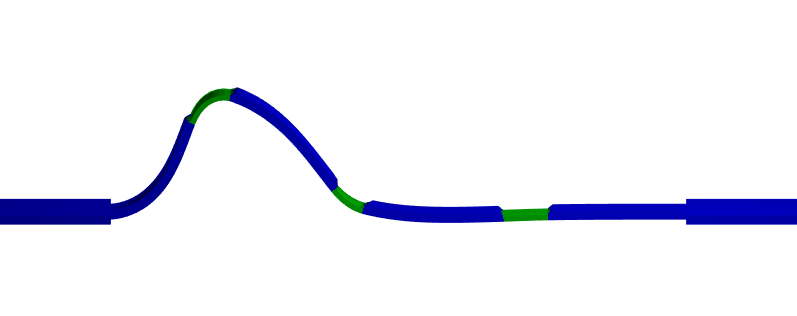
\includegraphics{tratio/2-0.56.png} & \xmark                          & \xmark \\
    0.46 & 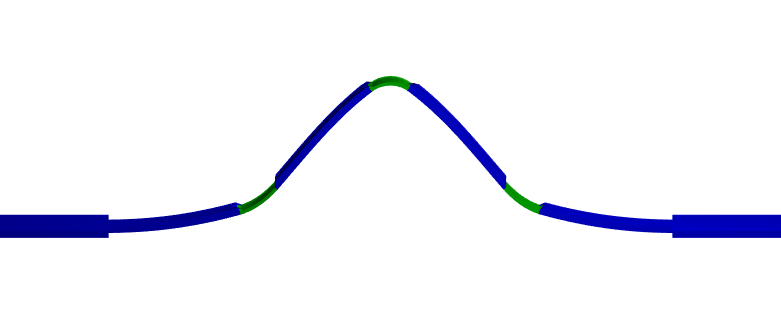
\includegraphics{tratio/1-0.46.png} & 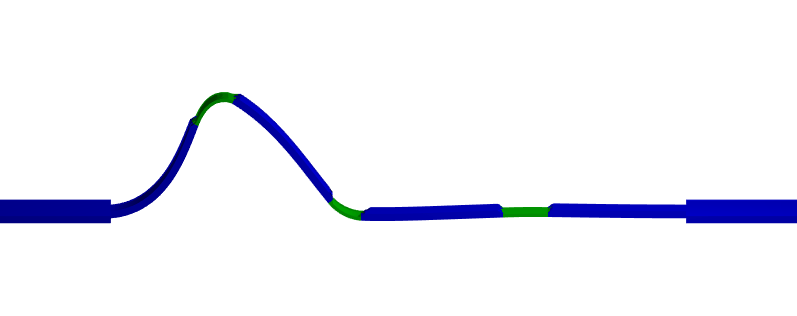
\includegraphics{tratio/2-0.46.png} & 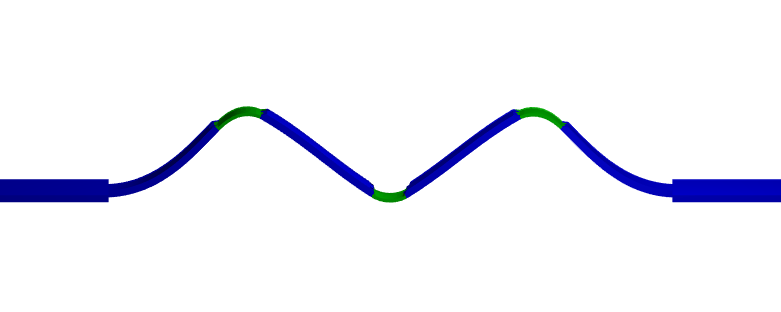
\includegraphics{tratio/3-0.46} & \xmark \\
    0.33 & 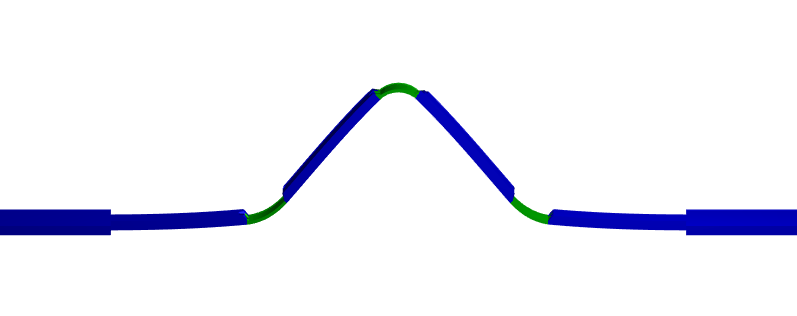
\includegraphics{tratio/1-0.33.png} & \xmark                              & 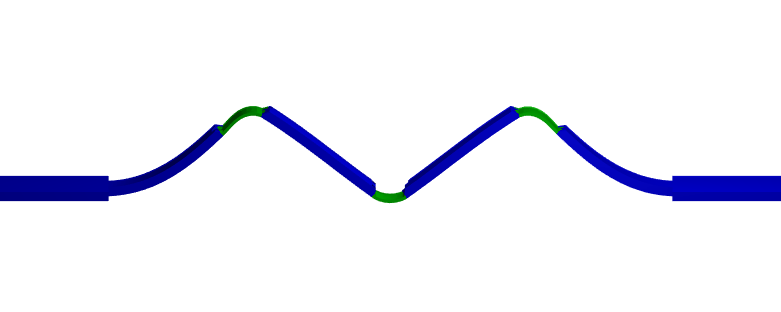
\includegraphics{tratio/3-0.33} & 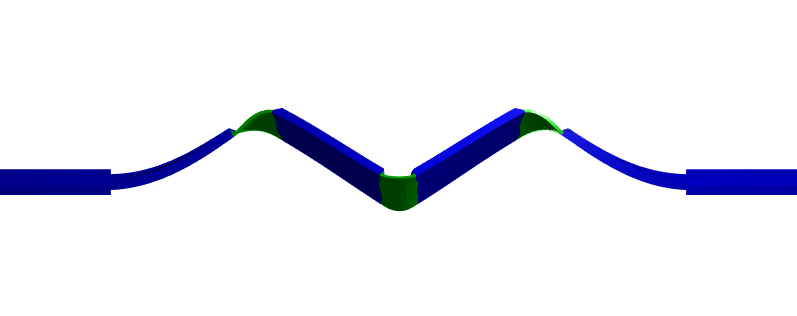
\includegraphics{tratio/4-0.33.png} \\
    0.25 & 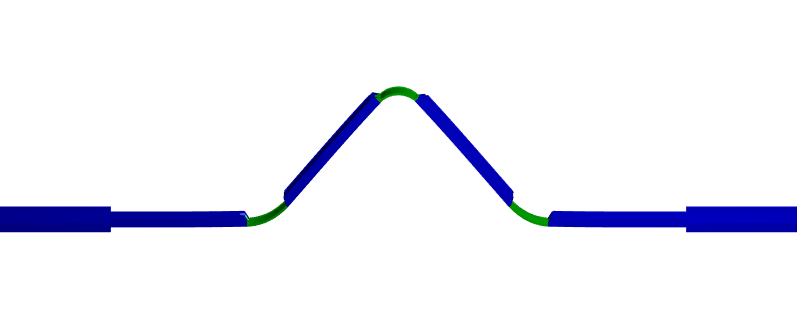
\includegraphics{tratio/1-0.25.png} & \xmark                              & 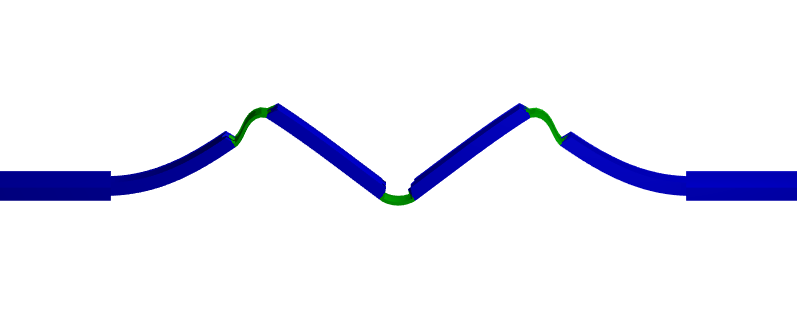
\includegraphics{tratio/3-0.25} & \xmark \\
    \hline
  \end{tabularx}
  \caption{Effect of the crease thickness ratio on the multistability of the ribbon structure (strain: 14\%; length ratio: 0.32)}
  \label{tab:or-S1}
\end{table}

\begin{table}[htb]
  \setkeys{Gin}{width=\linewidth}
  \begin{tabularx}{\textwidth}{CCCCC}
    \hline\hline
    Length ratio & State 1 & State 2 & State 3 & State 4 \\
    \hline
    0.10 & 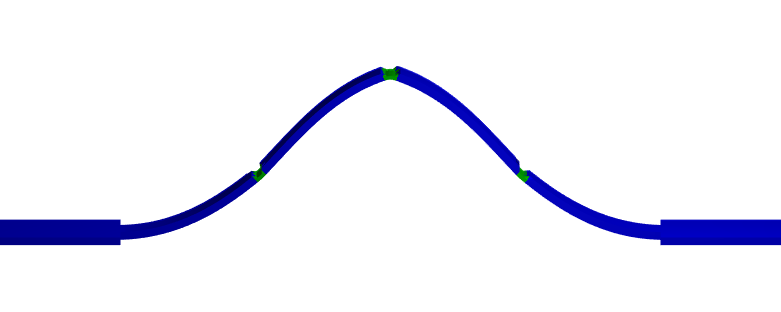
\includegraphics{lratio/1-0.1.png}  & \xmark                              & \xmark                          & \xmark \\
    0.18 & 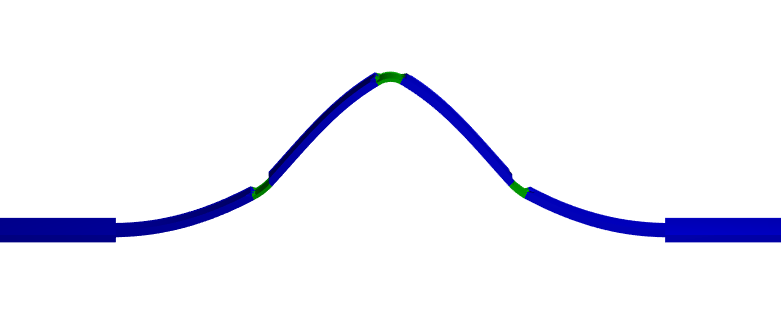
\includegraphics{lratio/1-0.18.png} & 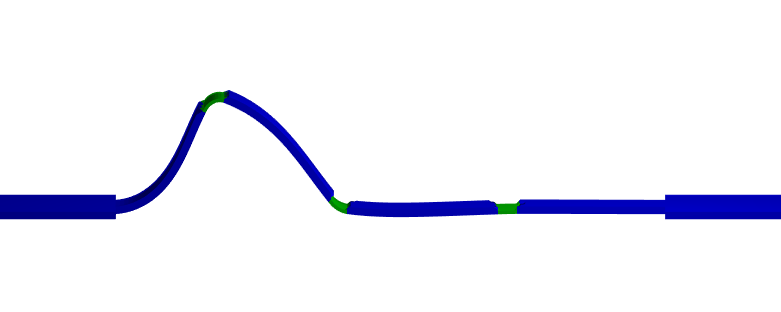
\includegraphics{lratio/2-0.18.png} & \xmark                          & \xmark \\
    0.32 & 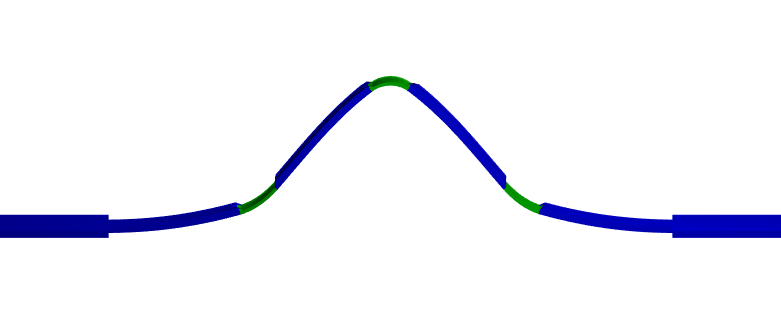
\includegraphics{lratio/1-0.32.png} & 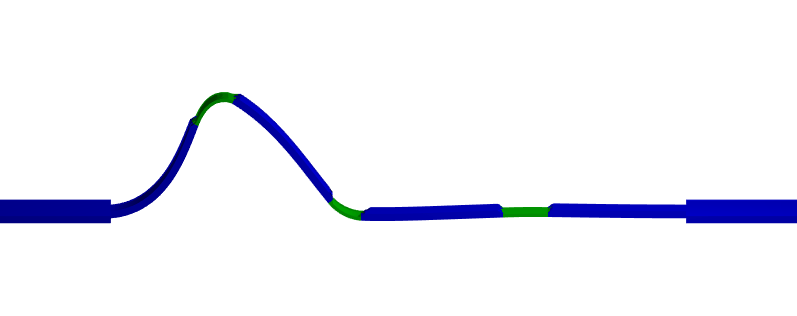
\includegraphics{lratio/2-0.32.png} & 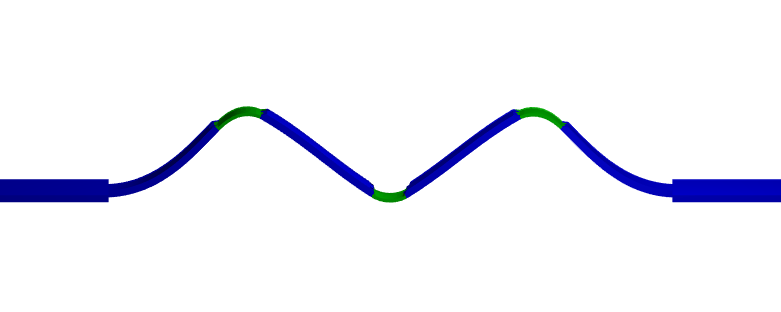
\includegraphics{lratio/3-0.32} & \xmark \\
    0.56 & 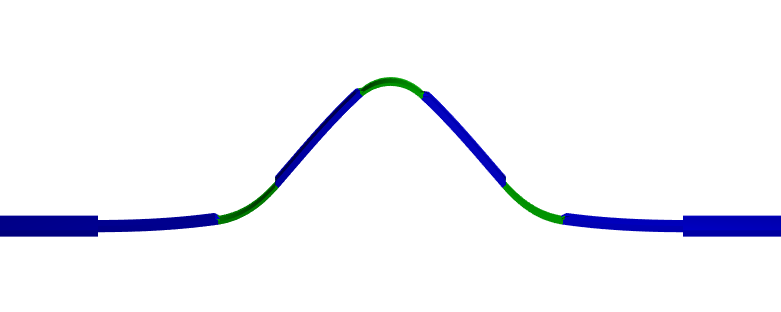
\includegraphics{lratio/1-0.56.png} & 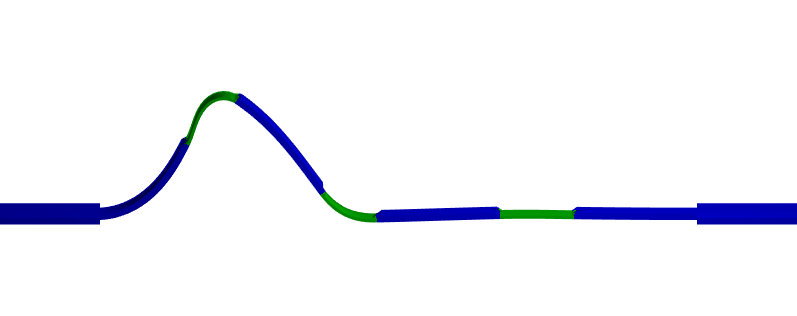
\includegraphics{lratio/2-0.56.png} & 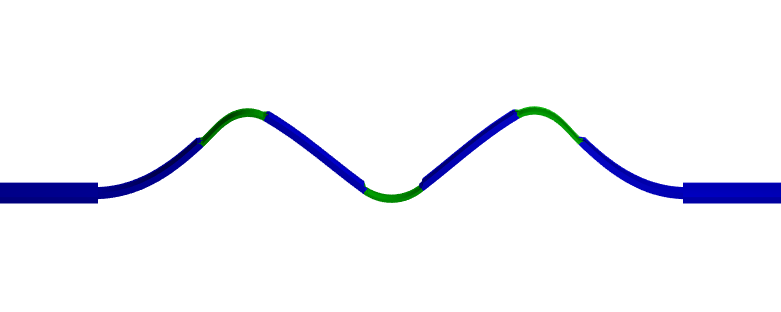
\includegraphics{lratio/3-0.56} & 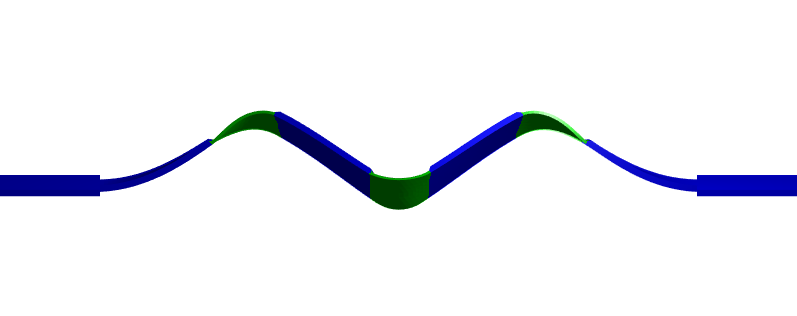
\includegraphics{lratio/4-0.56.png} \\
    1.00 & 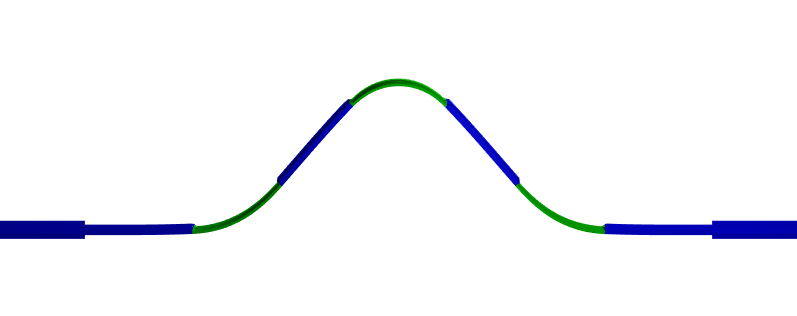
\includegraphics{lratio/1-1.png}    & \xmark                              & 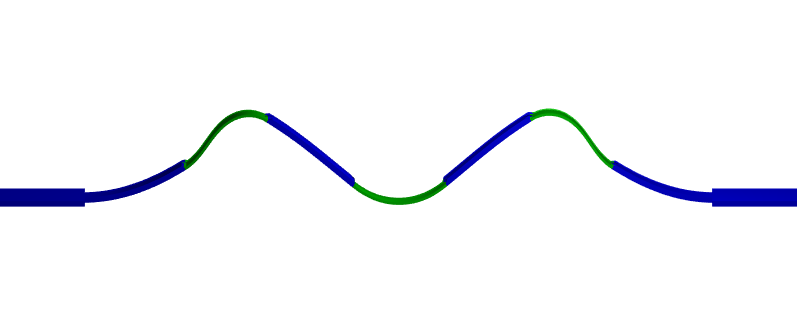
\includegraphics{lratio/3-1}  & 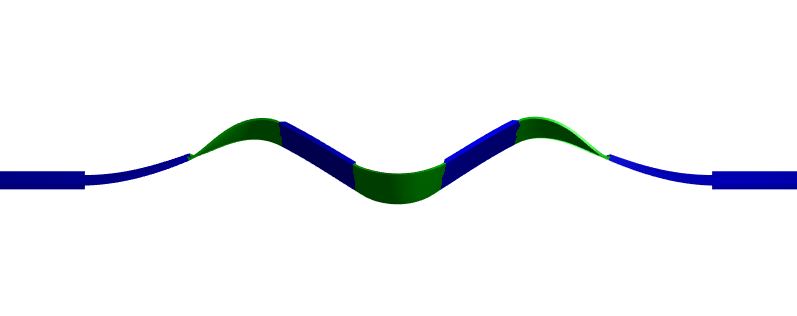
\includegraphics{lratio/4-1.png} \\
    \hline
  \end{tabularx}
  \caption{Effect of the crease length ratio on the multistability of the ribbon structure (strain: 14\%; thickness ratio: 0.46)}
  \label{tab:or-S2}
\end{table}

The results in \cref{tab:or-S1,tab:or-S2} show that both ratios can have a significant effect on the multistability of the ribbon structure.
In particular, reducing the crease thickness and increasing its length has an overall similar effect on the stable states as increasing the compressive strain.
The main difference is at the extreme when state 3 remains stable, rather than progressing to the twisted state.
This is because reducing the thickness of the crease, or increasing its length, grants the creases more flexibility, which reduces the amount of bending that is required in the edge segments.
However, it is likely that at larger compressive strains state 3 will become unstable.


\subsection{Reconfiguration pathways for a 3-crease ribbon structure} \label{sec:or-paths}

In addition to locating the stable configurations, we also investigate available pathways that the structure can be reconfigured among its stable states, which is important for many applications.
The pathways have been computed using the same method as \cref{ch:mesostructures}, first by finding the TS with BITSS, for which the separation of the two states is reduced by 30\% each iteration, and then computing the pathways using a combination of downhill minimisation and the string method.
In addition, once a transition state is found for a given strain, a continuation approach is then used with the BITSS method in order to identify the energy barriers across the whole range of strains that the pathway exists.

\begin{figure}
  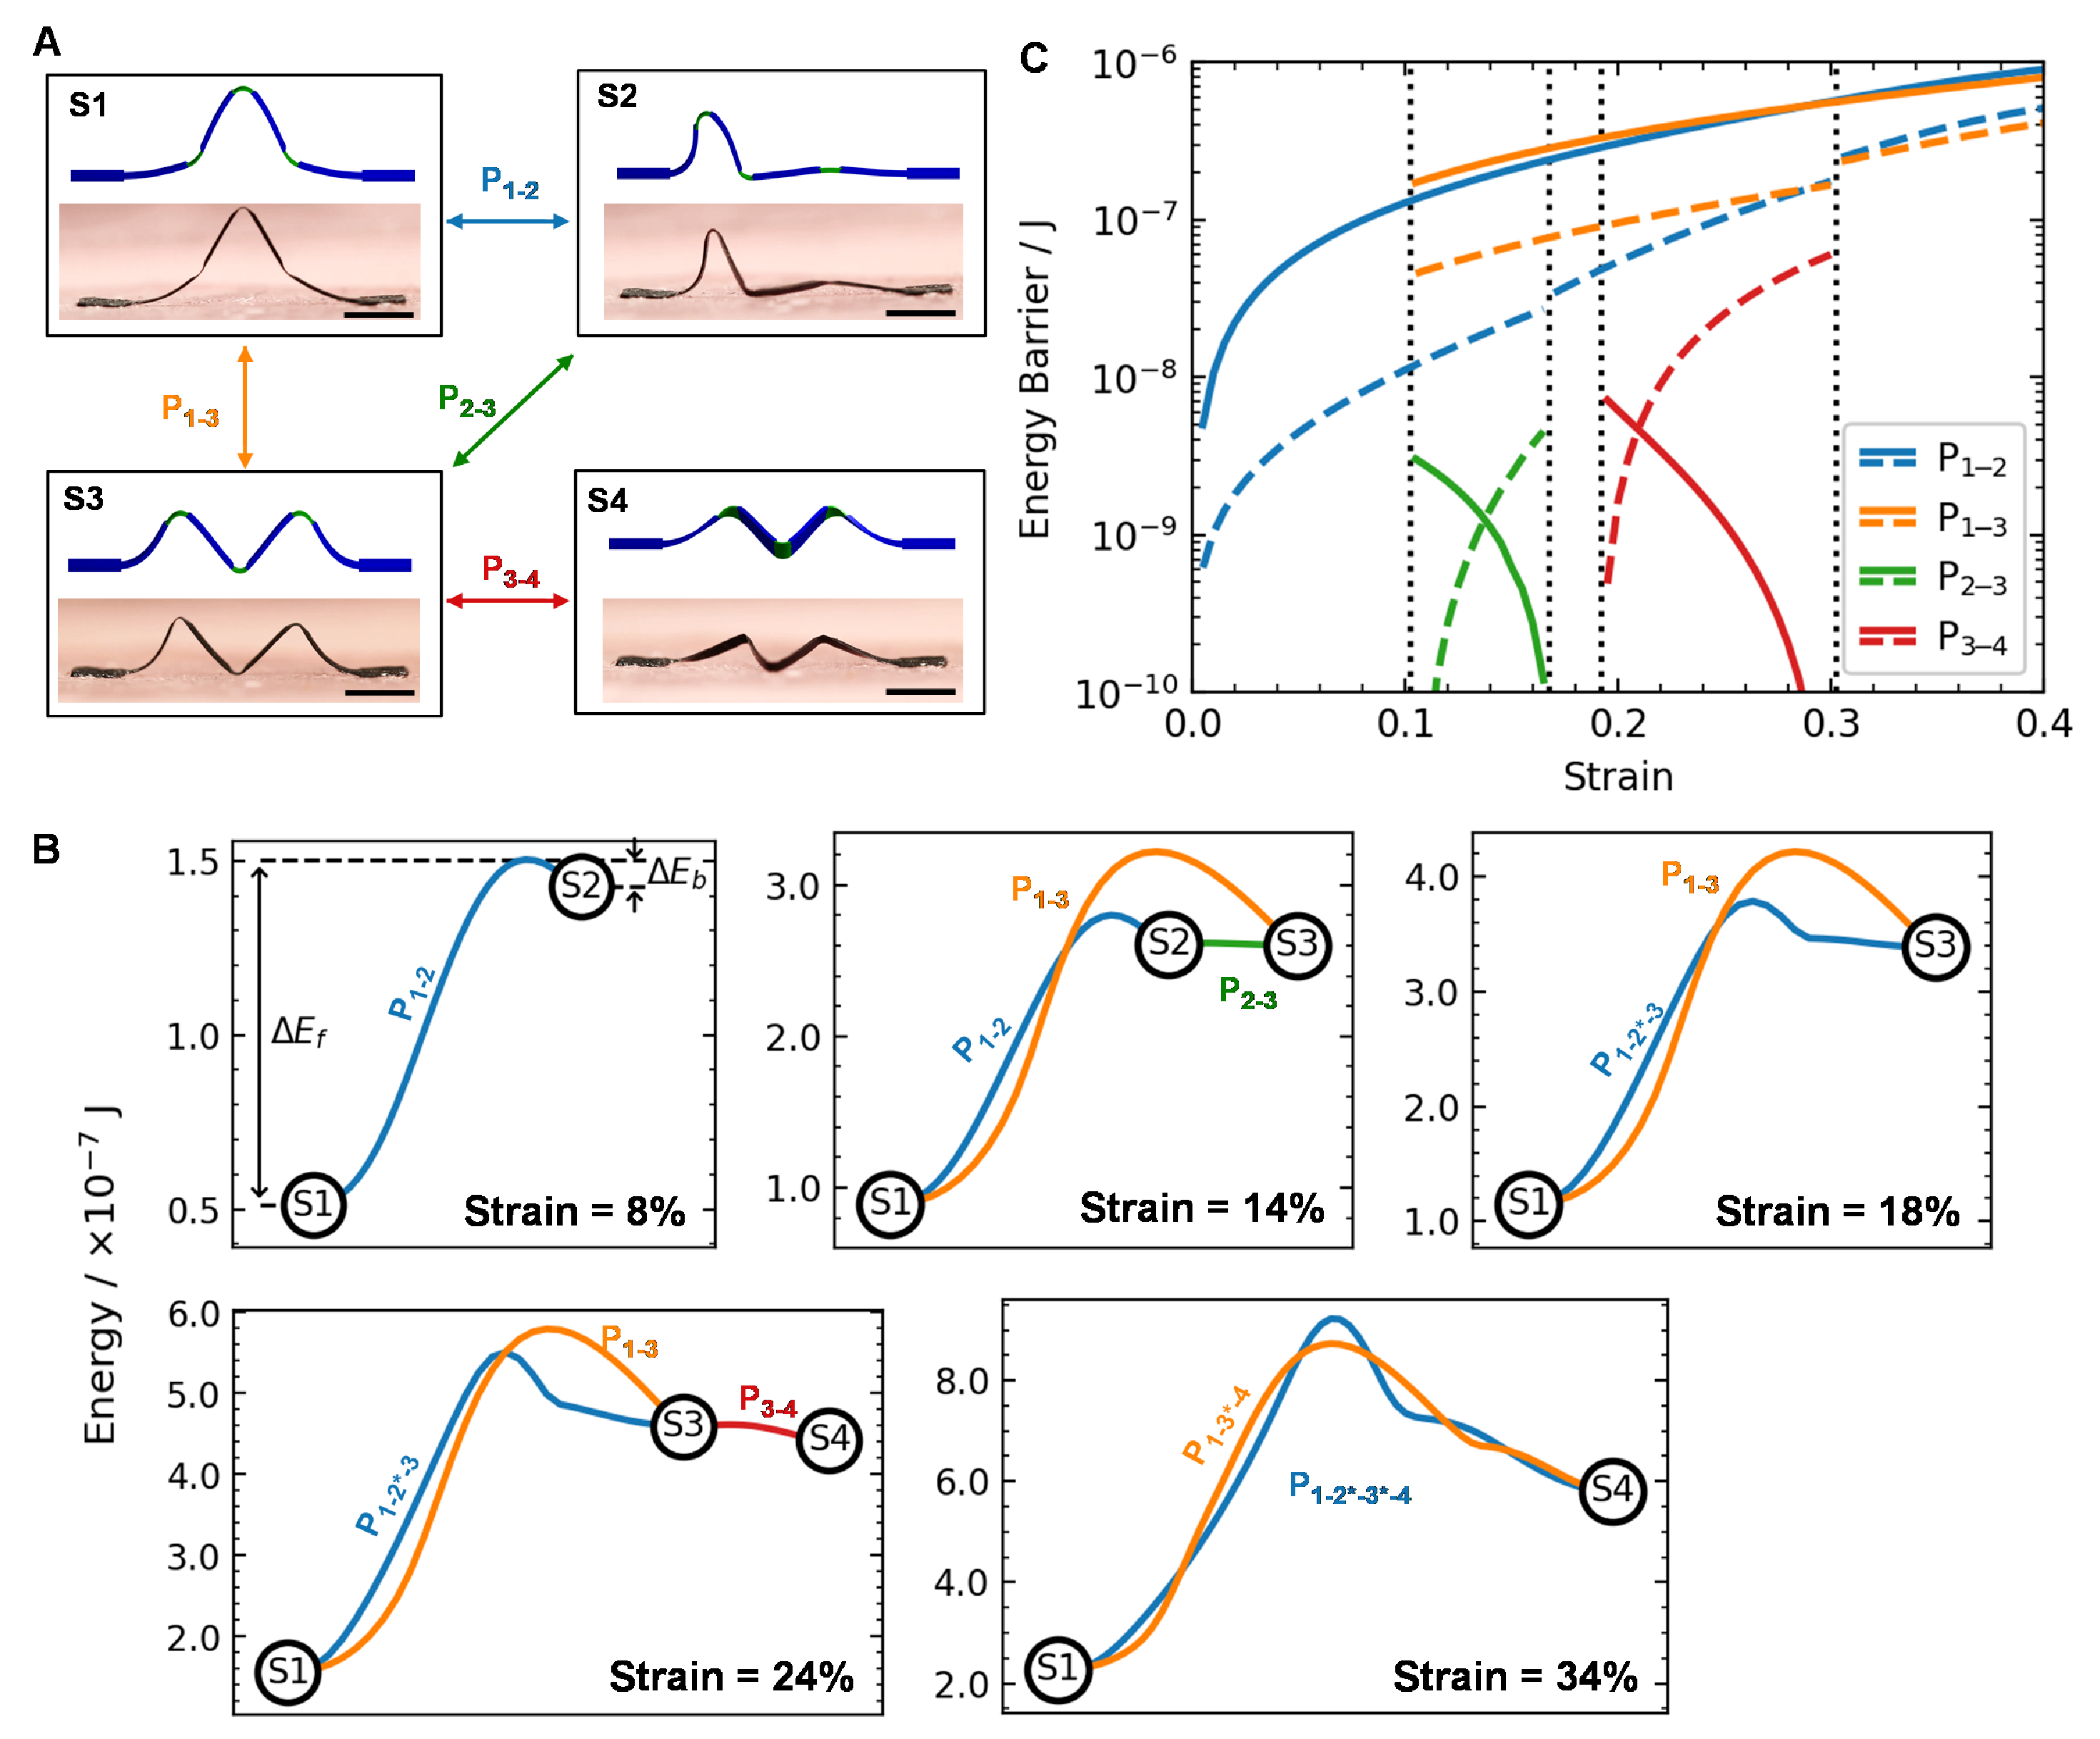
\includegraphics[width=\textwidth]{figure_3.pdf}
  \caption{
    (A) Reconfiguration paths among the distinct stable states of origami-inspired ferromagnetic ribbon structures.
    Scale bars, 2 mm.
    (B) Energy profiles of pathways for the 3-crease ribbon structure at various strain levels. (C) Minimum energy barriers for pathways in \cref{fig:or-2}(b) as a function of the strain.
    The solid lines indicate the energy barriers from the lower numbered states to the higher numbered states  and the dashed lines are the barriers from the higher numbered states to the lowered numbered states (illustrated by $\upDelta E_f$ and $\upDelta E_b$ in \cref{fig:or-3}(b), respectively) .
    The line colors correspond those in \cref{fig:or-3}(a).
    The blue and orange lines also encompass the extended pathways P\textsubscript{1-2*-3}, P\textsubscript{1-2*-3*-4}, and P\textsubscript{1-3*-4}.
  }
  \label{fig:or-3}
\end{figure}

Here we use the three-crease structure as a representative case for study because of its complexity in the configurations and the number of stable states, which results in a large number of reconfiguration paths.
As illustrated in \cref{fig:or-3}(a), we identify four distinct pathways among the stable states of the structure: P\textsubscript{1-2} for the transition path between S1 and S2, P\textsubscript{1-3} between S1 and S3, P\textsubscript{2-3} between S2 and S3, and P\textsubscript{3-4} between S3 and S4.
It is worth noting that in cases where one or more of those states are not stable, the corresponding individual paths may merge into one, as we will detail below.

\Cref{fig:or-3}(b) shows the available pathways and the associated energy profiles for a representative case in each of the five regimes for a 3-crease ribbon (identified in \cref{fig:or-2}(a)) as the strain is increased from 0\% to 40\%.
In the first regime (0-10\% strain), only states S1 and S2 exist, with a single pathway (P\textsubscript{1-2}) to reconfigure between them, as shown in \cref{vid:ribbon8}.
In the second regime (10\%-17\% strain), state S3 appears, so two additional pathways, P\textsubscript{1-3} and P\textsubscript{2-3}, become accessible (\cref{vid:ribbon14}).

Our analysis also highlights that there are not only multiple stable states existing in the structure, but also multiple available paths for transforming the structure from one state to another.
For example, we can observe that there are two main pathways that can be taken from state S1 to S3.
The first path, initially following P\textsubscript{1-2} to reconfigure S1 to S2, subsequently involves the creation of an asymmetric peak at one side of the structure to form state S3 from S2 (P\textsubscript{2-3}).
Due to symmetry, there are two equivalent scenarios depending on which side the peak is created to form S3.
The second path, P\textsubscript{1-3}, directly reconfigures S1 to S3 by forming two edge peaks simultaneously while maintaining symmetry.

As the strain increases to the regime of 17\%-19\%, state S2 becomes unstable, so P\textsubscript{1-2} and P\textsubscript{2-3} merge into a single path P\textsubscript{1-2*-3} (\cref{vid:ribbon18}), where 2* denotes that state 2 is no longer stable.
Above the strain of 19\%, pathway P\textsubscript{3-4} appears between state S3 and twisted state S4, while the two pathways from S1 to S3 still exist (\cref{vid:ribbon24}).
Finally, at the strain of 30\% and above, S3 is no longer stable leaving just two merged paths P\textsubscript{1-2*-3*-4} and P\textsubscript{1-3*-4} between S1 and S4 (\cref{vid:ribbon34}).

We further investigate the energy barriers of each pathway as a function of strain.
For each pathway, there are two relevant energy barriers, as illustrated in \cref{fig:or-3}(b) using P\textsubscript{1-2} in the case of 8\% strain as an example.
We label $\upDelta E_f$  for the energy required to transition from a lowered numbered state to a higher numbered state in each pathway (here, S1 to S2), while $\upDelta E_b$ is the energy required for the opposite transition (here, S2 to S1).
We summarise the values of the energy barriers for all the available pathways in \cref{fig:or-3}(c), where $\upDelta E_f$ and $\upDelta E_b$ for each pathway are represented by solid and dotted lines, respectively.

We can see that the energy barriers for pathways reconfiguring from S1 to other states including S2, S3 and S4 depending on the strain levels (P\textsubscript{1-2}, P\textsubscript{1-2*-3}, P\textsubscript{1-2*-3*-4}, P\textsubscript{1-3}, P\textsubscript{1-3*-4}; solid blue and orange lines) are much larger than their corresponding reverse barriers (dotted blue and orange lines, respectively).
Such difference suggests that state S1 is more stable than the other states (S2, S3 and S4), which is consistent with the phase diagram in \cref{fig:or-2}(a), where S1 is almost always stable for cases under all crease numbers.

It is also seen that the energy barriers of paths P\textsubscript{2-3} and P\textsubscript{3-4} are significantly lower than those of pathways involving state S1.
This suggests that reconfigurations among states S2, S3, and S4 are much easier than those between S1 and S2/S3/S4.
Correspondingly, the required forces to disturb the reconfiguration paths or trap locally stable states are low.
Hence, forces like friction between the structure and the substrate (assembly platform) in experiments may be sufficient to trap the structure along these paths or at states S2, S3 and S4.
This may explain why experimentally the structure appears to get trapped in some states which are shown to be unstable in computational results (\cref{vid:ribbon18,vid:ribbon24,vid:ribbon34}).
For example, in \cref{vid:ribbon18}, when the structure is reconfigured from S2 to S3, the 2nd edge peak is not fully formed due to possible friction between the structure and the substrate, causing the slight asymmetric configuration of S3.

From \cref{fig:or-3}(c), we can also see that the energy barriers for the majority of the reconfiguration paths increase monotonically with the strain, implying that it becomes more difficult to reconfigure the states at larger strains.
Exceptions occur for reconfiguration paths P\textsubscript{2-3} (solid green line, transition from S2 to S3) and P\textsubscript{3-4} (solid red line, transition from S3 to S4), the energy barriers of which decrease with increasing strain levels.
Here, the cases when the energy barriers tend to be zero correspond to the instances where S2 and S3 become unstable, i.e., the instability modes of these states.
Overall, the energy barrier analysis reinforces the previous observation that, as the strain is varied from 0\% to 40\%, state S1 always exists while the availability of states S2, S3 and S4 strongly depends on the strain imposed.


\subsection{Multi-ribbon structures}\label{sec:or-structures}

The multistable ribbon configurations studied above can serve as building blocks for complicated geometries and diverse types of origami-inspired structures.
Several such structures are detailed in this section that have been created by our collaborators.

\Cref{fig:or-4}(a) show a $3\times3$ array of ribbons with three creases at different strain levels, which is consistent with the prediction of the phase diagram in \cref{fig:or-2}(a).
Particularly, as predicted by the phase diagram, three distinct stable states exist at the strain levels of 14\% (S1, S2, and S3) and 28\% (S1, S3, and S4), respectively.
In experiments, each individual ribbon unit is separately addressable and therefore the structure array can be magnetically tuned in a sequential manner to simultaneously display all the three stable states (S1 in row 1, S2 in row 2, and S3 in row 3 at a strain of 14\%; S1 in column 1, S3 in column 2, and S4 in column 3 at a strain of 28\%).
Such capability of dynamically and reversibly tuning the patterns in a structure array represents an important option for applications including digital coding and smart switches\cite{Chen2021}, especially when integrated with other functional materials or elements.

In addition, the complexity of origami-inspired structures and the number of stable states can be increased by incorporating a larger number of interconnected structural units, like ribbons with two creases.
\Cref{fig:or-4}(b) presents a structure consisting of two creased table structures connected with a creased ribbon, which can be magnetically reconfigured into six distinct stable states that are enabled by the multistability of the ribbon units.
Furthermore, the multistable origami-inspired structures can be extended to diverse geometries.
For example, \cref{fig:or-4}(c) demonstrates a structure that mimics insect flexion, with various standing states that show biomimetic movements.
Here the legs can be treated as two-crease ribbons with each switching between their two asymmetric cases (S2 in \cref{fig:or-2}).
When the peak is beside the binding site, it corresponds to the insect lying flat.
But if the peak is beside the body then it causes the insect to stand upright.

\begin{figure}
  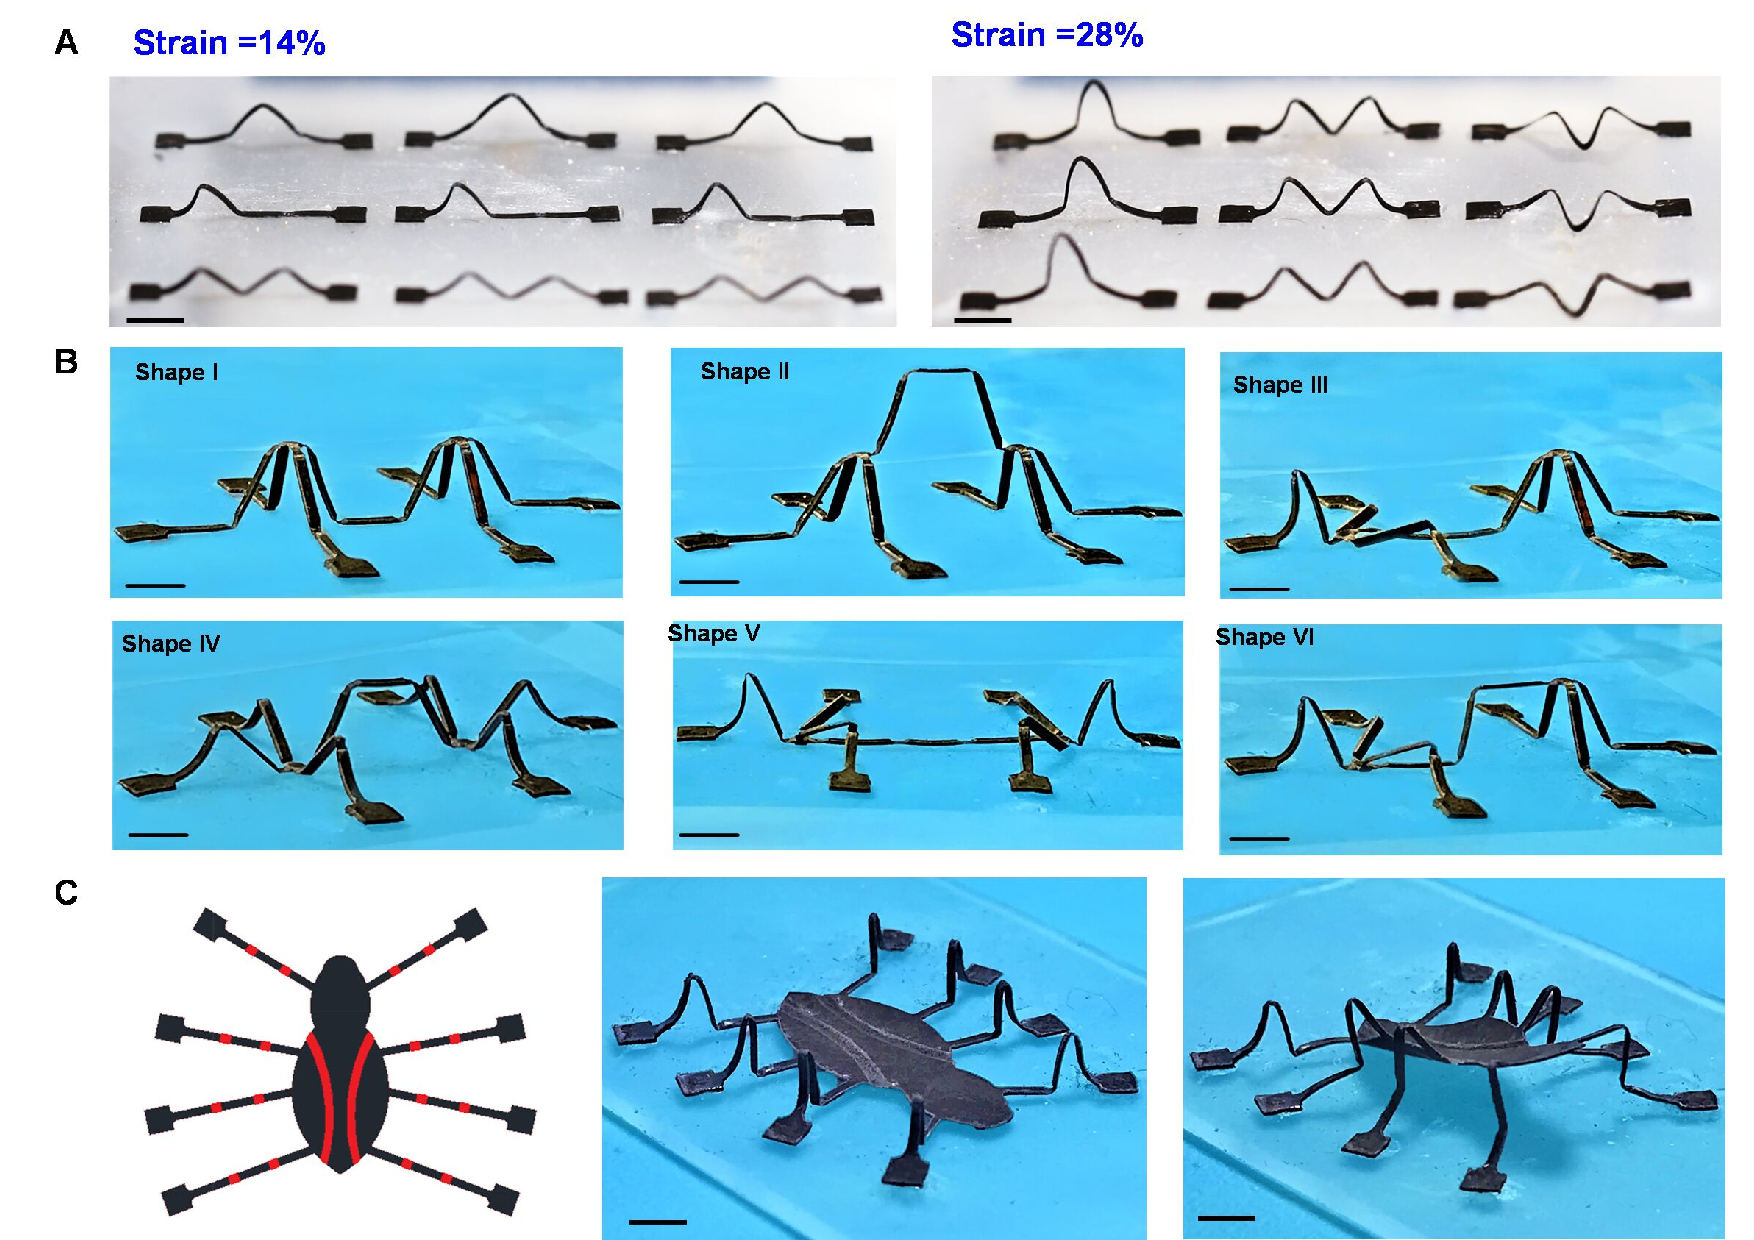
\includegraphics[width=\textwidth]{figure_4.pdf}
  \caption{
    Diverse origami-inspired, multistable ferromagnetic structures that can be actuated by magnetic forces.
    (A) An array of 3-crease ribbon structures showing different patterns formed by the multistable states of the ribbon under the strain of 14\% and 28\%, respectively.
    Scale bars, 3 mm.
    (B) Multistable states and magnetic reconfiguration of a double-table structure composed of creased ribbon segments.
    (C) A multistable biomimetic ``insect'' in its flat and standing states, respectively.
    Scale bars, 2 mm.
  }
  \label{fig:or-4}
\end{figure}



\section{Conclusion}

To sum up, it has been shown that the multistability and the associated transition paths of origami-inspired, compressively buckled ferromagnetic structures can be tailored by controlling the number of creases and assembly strain.
Our constructed phase diagram of a representative creased ribbon structure from the energy landscape analysis provides important guidelines for the targeted number of stable states by varying the two control factors.
In addition, transition pathways among the distinct stable states are computed and illustrate how the structure can be manipulated to be reconfigured along different pathways.
These have been validated using experimental results of origami-inspired ferromagnetic structures, which show targeted multistable states following designed pathways, which highly agree with modelling.

The fundamental understanding of the multistability of creased ribbon structures provides important guidelines for the design and application of multistable origami-inspired systems, with demonstrated examples including an arrays of creased ribbon units and the various states of a biomimetic ``insect'' structure.
Also, the energy landscape analysis offers an approach to study the multistable states and pathways, and can be tailored for specific applications.

These results highlight potential opportunities in the future to exploit multistable, origami-inspired ferromagnetic structures for intelligent and adaptive systems such as programmable logic array by integrating complex structure design and functional materials like stimuli-responsive polymers and electronics.
It will also be interesting to explore the concept of actively manipulating the number of stable states and their reconfiguration paths in the design of other types of functional structures by using alternative control parameters.

\begin{table}[]
  \begin{tabularx}{\textwidth}{>{\hsize=.3\hsize\linewidth=\hsize}C >{\hsize=.55\hsize\linewidth=\hsize}C >{\hsize=2.1\hsize\linewidth=\hsize}C >{\hsize=1.05\hsize\linewidth=\hsize}C}
    \hline\hline
    Topic & Symbol & Parameter description & Value \\
    \hline
    \multirow{8}{*}{\rotatebox[origin=c]{90}{Structure}}
          & $t$               & Thickness        & \SI{130}{\micro\metre} \\
          & $t_\text{crease}$ & Crease thickness & \SI{60}{\micro\metre} \\
          & $l$               & Segment length   & \SI{2.5}{\milli\metre} \\
          & $l_\text{crease}$ & Crease length    & \SI{0.8}{\milli\metre} \\
          & $w$               & Ribbon width     & \SI{0.8}{\milli\metre} \\
          & $\rho$            & Density          & \SI{2.59}{\gram\per\centi\meter\cubed} \\
          & $Y$               & Young's modulus  & \SI{1.4}{\mega\pascal} \\
          & $\nu$             & Poisson ratio    & 0.3 \\
    \hline
    \multirow{4}{*}{\rotatebox[origin=c]{90}{L-BFGS}}
          & $m$  & Iteration memory             & 5 \\
          & ---  & Initialisation iterations    & \num{30000} \\
          & ---  & Initialisation force density & \SI{10}{\newton\per\meter\squared} \\
          & ---  & Gradient RMS convergence     & $10^{-11}$ \\
    \hline
    \multirow{6}{*}{\rotatebox[origin=c]{90}{Pathways}}
          & $\alpha$ & BITSS energy constraint strength    & 10 \\
          & $\beta$  & BITSS distance constraint error     & 0.1 \\
          & $f$      & BITSS distance reduction factor     & 0.2 \\    
          & ---      & BITSS coefficient regularity        & 100 iterations \\    
          & ---      & String reparametrisation regularity & 5000 iterations \\
          & ---      & String number of images             & 60 \\
    \hline\hline
  \end{tabularx}
  \caption{\label{tab:or-params}
    Values of the parameters that are used throughout this chapter, unless otherwise specified.
  }
\end{table}
